\documentclass[11pt, rgb, twoside, bibtotoc]{scrreprt}
\usepackage{themeKonstanzDBIS} % Muss immer verwendet werden (Standardpaket)
\format{a4tufte}

% Thesis information        %
\date{\today}
\year{2019}
\author{Fabian Klopfer}
\title{Label Hierarchy Inference in Property Graph Databases}
\subtitle{Bachelor Thesis}
\unisection{Faculty of Sciences}
\department{Department of Computer and Information Science}
\supervisorOne{Prof. Dr. Michael Grossniklaus}
\supervisorTwo{Prof. Dr. Tatjana Petrov}

\headFoot{12}
\bibliography{resources}

\begin{document}

% Keep the focus
% Sell yourself (what was hard,...)
% dont overdo it 

% Makro für nicht gefundene zitationen mit warning wenn unbedingt nötig
% sonst todo

% Related work separate
% Dont overdo it, dont define too much notation
% KISS, only use notation when needed extensively
% Related work: project stuff and why not working; onnly competitors that do the same thing
% bachground 
% Write about EVERYTHING: Methods include all the bachelor project things

\newgeometry{left=2.5cm, right=2.5cm, bottom=2cm, top=2.5cm, headheight=12pt, headsep=0.8cm, footskip=22pt}
% Schmutztitel als poster
\thesistitlepage[language=english]{Bachelor Thesis}
\newpage
\cleardoublepage
% Table of Contents           
\tableofcontents

\restoregeometry
\cleardoublepage

\rmfamily 
\normalsize

\chapter{Introduction}
Use mixture of Michalski, Fisher, Han, Mirkin, Jain, Berkhin, Concept formation in psychology rosch, gluck, corter,..., trestle, query optimizazion for un or semi structured databases

\section{Contributions}
NOTICE CONTRIBUTIONS CLEARLY: 
1. SURVEY \& EVALUATION OF CLUSTERING ALGORITHMS
2. MULTI-PHASE CLUSTERING WITH DENDROGRAM FLATTENIONG
2.1 occurence of problems, noise, ... solution is 3.
3. IMPLEMENTATION OF CONCEPTUAL CLUSTERING/COBWEB
4. ADAPTION TO GRAPH SCENARIO, GENERALIZATION OF PROPERTY CONTAINERS IN THE GRAPH
5. FLEXIBILITY OF THE PIPELINE, POSSIBLE EXTENSIONS TO SUPPORT QUERY OPTIMIZATION 

Theodoros: more? less? what are the contributions and how to make it shiny but not too shiny
\section{Outline}
2. background
3. clustering algorithms \& features  (related work)
4. Pipeline for multiphase and graph aware clustering to obtain hierarchical concept descriptionhs
5. evaluation
6. conclusion
\chapter{Background}\label{\positionnumber} 

\section{Property Graph Model}\label{\positionnumber}
A \textbf{Property Graph} is a 9-Tuple $G = (V, E, \lambda, P, T, L, f_P, f_T, f_L)$ with 
\begin{itemize}
    \item $V$ the set of vertices of the graph.
    \item $E \subseteq (V \times V)$ the set of edges of the graph.
    \item $\lambda: E \rightarrow $ a non-reflexive\note{i.e. the edges are directed. \\
    If the graph was directed $\lambda$ would be a reflexive function. \\
    Normally in a graph the edges $E \subseteq (V \times V)$ but in the property graph model edges have sets of properties, thus making them objects on their own.\vspace{1cm}}
 function assigning a pair of nodes to an edge.
    \item $L$ a set of strings used as labels.
    \item $P$ a set of key-value pairs of type String, Value\note{the actual supported types of values depend on the implementation} called properties.
    \item $T$ a set of strings used as relationship types.
    \item $f_P: V \cup E \rightarrow 2^P$ a function that assigns a set of properties to a node or relationship.
   \item $f_T: R \rightarrow T$ a function that assigns a type to  a relationship.
   \item  $f_L: N \rightarrow 2^L$ a function that assigns a node a set of labels.
\end{itemize} 
\smallskip
The property graph model reflects a directed, node-labeled and relationship-typed multi-graph $G$, where each node and relationship can hold a set of key-value pairs \cite{angles2018property}. An illustration of this model is shown in fig. \ref{fig:propertygraph}\fig{img/property_graph_elements.jpg}{propertygraph}{A visualization of the property graph model}{1}.
Neo4J is a graph data base employing the property graph model~\cite{neo4j_book}, which is used in the evaluation part of this thesis.


\section{Cluster Analysis}\label{\positionnumber}
Clustering or Cluster Analysis is defined by the automated process of splitting the set of observations into subsets, in order to group them such that objects in different subsets are different from another and objects within a subset are as similar~\cite{han2011data}. \\
According to Mirkin, "Clustering is a mathematical technique designed for revealing classification structures in the data collected on real-world phenomena"\cite{mirkin2013mathematical}, with the purpose of analyzing structure in the data, relate different aspects and assist in designing classification schemes. 
Let $O$  be the set of data objects\note{or equivalently data instance, data point, data sample} \\
Let $O_0, O_1, \dots, O_n \subset O$ with
\begin{itemize}
    \item $\forall i \in \{0, 1, \dots n\}: \cup_i O_i = O \wedge$
    \item $\forall i \in \{0, 1, \dots n\} \forall j \in \{0, 1, \dots n\}\setminus\{i\}: O_i \cap O_j =\emptyset$
\end{itemize}
Then $O_0, O_1, \dots, O_n$ is a clustering of $O$. \\
Each subset $O_i$ of the subset is called a cluster and clusters may or may not overlap. Thus the goal of a clustering algorithm is to find a set of subsets that optimize an objective function based on the attributes and values $A, V$. Note that the term clustering only imposes an order on the objects and not on the attributes. The constraints defined on the set of attributes and values is imposed by the objective function of the respective algorithm. \\

Depending on the method used and the objective that is optimized for, the clustering differs between different algorithms. \\

In order to compute any metric or to find similarities and differences or patterns in the set of objects, they must have some attributes, i.e. $A \neq \emptyset, V \neq \emptyset$ and a relation $I$ mapping Objects to Atrributes and their respective value\note{If no object has an attribute the only logic clusterings are the trivial ones: \begin{itemize}
    \item $O_0 \equiv O \wedge \forall i \in \{1, \dots n\}: O_i \equiv \emptyset$
    \item $\forall i \in \{0, 1, \dots n\}: |O_i| = 1 \wedge \sum_i |O_i| = |O|$
\end{itemize}}.
Thus all algorithms can be defined by the following interface:
\begin{algorithm}[h]
    \KwIn{The Relation $I$ that maps objects to attributes and values }
    \Parameters{Parameters P to the implementation if necessary}
    \KwOut{A set of subsets$O: O_0, O_1, \dots, O_n$} 
\caption{Clustering Algorithm}\label{clustering}
\end{algorithm}
Often clustering algorithms only consider feature vectors, i.e. only consider the relation $I$ in the nominal case or $V, I$ in the numeric case. Clustering may thus be seen as a partial form of Formal Concept Analysis\note{For an introduction to Formal Concept Analysis, see \autoref{7.1}}, as it's approach may be less strict in terms of attribute restrictions, may have a one-sided focus on objects in terms of connections - contrary to the Galois connections used in Formal Concept Analysis and lattice theory - and partial as many clustering algorithms only split the input once into a set of subsets instead of exploring all sets for a given rule recursively.
There are also algorithms constructing Concept lattices, but those may be too restrictive for noisy applications and exponential in run time\cite{doi:10.1111/j.1467-8640.1995.tb00031.x}. A class of clustering algorithms called hierarchical clustering algorithms is in the latter respect more similar to Formal Concept Analysis as sets of hierarchically ordered clusters are constructed.
The second class of clustering algorithms is non-hierarchic and produces so called flat clusters, i.e. only one partition level. This distinction between hierarchical and non-hoerarchical approaches is a narrow view on the wide field of clustering algorithms, a brief but broader overview is given in the following.

\subsection{Approaches}\label{\positionnumber}
Different surveys list different taxonomies and categories of clustering algorithms. In the following we are going to consider the ones discussed in \cite{han2011data} and \cite{overview_clust}.
% TODO Redo yourself, applied to used methods
\fig{img/taxonomy_clustering_han.png}{taxonomy_han}{A taxonomy of clustering algorithms and some examples for each class according to Han et al.~\cite{han2011data}}{1}
Han et al. compares the different methods by the representations used for data. Emphasizing that the proposed categories overlap, they define the following ones, depicted in fig. \ref{fig:taxonomy_han}\note{There are further classes like bi-clustering, evolutionary approaches and grid-based methods. Those are not used in the present work, but a breif description is provided in the appendix}:
\begin{itemize}
    \item \textbf{Partitioning methods:} Partition the objects into k disjoint groups. The input is partitioned only once producing a flat clustering. The requirement of disjoint groups may be relax for fuzzy clustering and related methods. Many partitioning algorithms use distance-based semantics, comparing the set of attributes of an object $A_{o}$ element-wise, calculating the distance between those values with respect to a certain scale and metric\note{e.g. Minkowski-distance for numeric attributes that may be interpreted geometrically as points in a space~\cite{THEODORIDIS2009701} or Jaccard-distance for a set of binary attributes~\cite{DBLP:journals/corr/Kosub16}}. Often partition-based methods use one or more prototypes to compare to when assigning a cluster to an object and tend to find rather spherically shaped clusters. \\
    
    \item \textbf{Hierarchical methods:} Merges (agglomerative) or splits (divisive) sets of objects recursively until all objects are assigned once in each level of the tree. Classic linkage-based approaches produce so called dendrograms \marginfigure{img/dendro_ex.png}{exdendro}{An example dendrogram.~\cite{dendroex}}{0cm} For an example see fig. \ref{fig:exdendro}. Hierarcical clustering can also be applied as a post-processing step of other methods in order to construct a hierarchy, which is one of the things that will be applied in the later chapters. \\
    
    \item \textbf{Density-based methods} use a combination of distance and neighbourhood to identify dense regions which are recognized as clusters, separated by less dense regions. Density-based methods may recognize outliers (single objects in low density regions) and naturally assign a quality measure to each cluster - it's density. Most density based methods produce flat clusters but there are extensions that append hierarchical clustering at the end to provide hierarchies (e.g. OPTICS and HDBSCAN), which will be elaborated on further in the former part of chapter 3. Also these methods are able to find not only spherical but arbitrarily shaped clusters.  \\
    
    \item \textbf{Model-based methods} are all approaches that use or construct a model to cluster instances. An example is the Gaussian Mixture Model that is the most common variant used with expectation maximization to estimate the mean and varience or in different terms the center and radius of blob-shaped clusters. In this category are also Self-Organizing Maps and other neural network-based approaches, as all these assume a certain model how the neurons shall learn weights between layers.  \\
    Another class of methods that is model-oriented are the conceptual clustering algorithms, first introduced by Stepp and Michalski~\cite{michalski1983learning}. Conceptual clustering algorithms construct a description along with the clustering of objects. We will focus on this method in the latter part of chapter 3.
\end{itemize}


\subsection{Clustering as a Search}\label{\positionnumber}
Clustering may be defined as a search for some set of subsets, dividing the input to satisfy some condition or optimizing for a certain metric function e.g. intra-cluster homogeneity and inter-cluster diversity~\cite{Fisher1987}. \\
\textbf{Search-based methods} improve \textit{incrementally} with every iteration on a certain objective function. Search-based methods are generally all methods that optimize an objective function, but emphasize the nature of the problem as being a search for certain solution. Many clustering algorithms are also search-based, i.e. try to find an optimal solution. \\
The search space is defined as the power set $2^O$ of the set of all Objects for flat clustering, and in case of hierarchical clustering the power set of each cluster of the tree besides the bottom-most layer\note{that is the layer that has single data instances as clusters}. An example for the former is K-Means, improving the quality of the chosen centroids of the clusters with each iteration. An example for the latter is Cobweb, where in each iteration the category utility is improved. A more concise description of the algorithms is given in the next chapter.

\section{Taxonomy}\label{\positionnumber}
Taxonomies\note{sometimes also referred to as concept hierarchy} organize observations into hierarchical classification schemes. A Taxonomy groups a set of objects depending on their properties and are able to represent sub- and super-ordinations as well as inheritance. An example are biological taxonomies, grouping animnals and plants into domains, Kingdoms, Phyla, Classes, and so on~\cite{Krcmar2015, han2011data}. A Taxonomy can also be seen as a hierarchy of labels, associated with certain concepts. \\
\marginfigure{img/taxonomy_ex.png}{taxonomy}{This graph scetches the main taxonomic ranks in biology \cite{TaxonomicRankGraph}}{-2cm}
More formally a taxonomy can be defined as sets of well-structured hierarchically ordered clusters. The term well-structured means here well-structured according to the practical application. E.g. a taxonomy of animals where each hierarchically ordered cluster only contains one element less as the above would be hierarchically ordered but not convenient in practice. A dendrogram is such a hierarchy that is not a usable taxonomy.

\section{Probability Theory}\label{\positionnumber}
Probability theory is essential to understand and implement probabilistic model-based approaches like COBWEB~\cite{Fisher1987} and will be used in chapters 3 to 5. \\
There are many textbooks extensively defining the notations needed in probability theory~\cite{Baron:2013:PSC:2536837, fahrmeir2016statistik}. The following is a summary of the most important terms used in the latter chapters.\\

A \textbf{sample space $\Omega$} is the set of all possible atomic results or outcomes of an experiment. An \textbf{event E} is a subset of the sample space, i.e. a set of elementary results or outcomes\note{As an example the a match day of a soccer league. Each match day 2n teams compete in n matches. The sample space would be all possible results $\Omega = \{ (i,j)| \forall i,j \in \mathbf{N}\}$. An event would e.g. be the set of results of a match day or a partial result.}.  \\

A \textbf{$\sigma$-algebra} on sample space $\Omega$ is a collection of events $\mathfrak{E} \subseteq 2^{\Omega}$ is a pair $(\Omega, \mathfrak{E})$ with
\begin{enumerate}
    \item $\Omega \in \mathfrak{E}$
    \item $E \in \Omega: E \in \mathfrak{E} \Rightarrow \Omega \setminus E \in \mathfrak{E}$
    \item $E_0, E_1, \dots \in \mathfrak{E} \Rightarrow E_0 \cup E_1 \cup \dots \in \mathfrak{E}$
\end{enumerate}
The pair $(\Omega, \mathfrak{E})$ is then called measurable space. \\

A \textbf{probability space $\mathcal{P} = (\Omega, \mathfrak{E}, P)$} is a structure with
\begin{enumerate}
    \item $(\Omega, \mathfrak{E})$ is a $\sigma$-Algebra
    \item $\forall x \in \Omega: 0 \leq P(x) \leq 1$
    \item $P(\Omega) = 1$
    \item $\forall i \geq 0 \wedge i \neq j: E_i \cap E_j = \emptyset: P(\cup_i E_i) = \sum_i P(E_i)$ 
\end{enumerate}
$P$ is called the \textbf{probability measure}.
\vspace{0.5cm}
A \textbf{discrete probability space} is a probability space $(\Omega, \mathfrak{E}, P)$ where 
\[ \exists E \subseteq \Omega: \forall e \in E: \{e\} \in \mathfrak{E} \wedge \sum_{e \in E} P(\{e\}) = 1\]
If the probability space is not discrete, it is called \textbf{continuous}. \\

A \textbf{measurable function $f:\Omega_0 \rightarrow \Omega_1$} is a function that maps a sample space of a measurable space $(\Omega_0, \mathfrak{E}_0)$ to another sample space of another measurable space $(\Omega_1, \mathfrak{E}_1)$ with:
\[ \forall E \in \mathfrak{E}: f^{-1}(E) = \{ e | f(e) \in E \} \in \mathfrak{E} \]

A \textbf{random variable $X: \Omega \rightarrow \mathbf{R}$} is a measurable function that maps a sample space to the real numbers. \\
The \textbf{Probability distribution $P_X$} of X is given by \[ P_X = P \circ X^{-1} \]

A \textbf{distribution function $F_X$}\note{Also called probability mass function for discrete probability space or cumulative density function for continuous probability spaces} of a random variable X is given by \[ x \in \mathbf{R}: F_X(x) = P(\{e \in \Omega | X(e) \leq x\}) \]
For the discrete case it can be formulated as: \[ x \in \mathbf{R}: F_X(x) = \sum_{x_i \leq x} P_x (X = x_i) \]
In the continuous case with $f$ the probability density function: \[ x \in \mathbf{R}: F_X(x) = \int^d f_X(x) dx \]

The \textbf{expected value $E[X]$}\note{Also known as the mean value.} is defined as the average of all possible outcomes, weighted by the respective probability to occur.
In the case of a discrete random variable: \[ \mu = E[X] = \sum_{x_i} x_i P(X=x_i)  \]
In the case of a continuous random variable: \[ \mu = E[X] = \int_{\mathbf{R}} x_i f_X(x_i)dx_i  \]

The \textbf{variance} may then be defined by \[ \sigma^2 = \text{Var}[X] = E[X^2] - (E[X])^2 \]

The \textbf{Gaussian distribution} is a continuous probability distribution with probability density function \[ f(x | \mu, \sigma^2) = \frac{1}{\sqrt{2 \pi \sigma^2}e^{-\frac{(x-\mu)^2}{2\sigma^2}}} \]
Notice that the Gaussian distribution can be identified in terms of mean and variance.

\chapter{Algorithm Selection}\label{\positionnumber}
% TODO use examples from presentation & yelp dataset
\section{Problem Statement}\label{\positionnumber}
A lot of data contains implicit regularities and structure~\cite{mitchell2006discipline}~\cite{carlsson2009topology} that are not reflected explicitly by the data model.\\
When focusing on data objects\note{or data instances, data points, elements of the sample, $\dots$} or nodes in terms of the property graph model there is often an implicit hierarchy of sub-types given a label. Such an implicit type hierarchy may provide further insights about the data as it may e.g. help in estimating cardinalities during query optimization, when keeping further statistics about the latent class distribution. \\

\margincode{code/business_ex.json}{businesex}{An example business object from the yelp data set}{text}{1cm}

For example in the yelp data set, the businesses may be further categorized in e.g. restaurants, spas, shopping malls, etc. One may further subdivide the restaurants by additional properties and features like cooking style (italian, asian, burgers, $\dots$) or  by location (italian restaurants in New York, asian restaurants in Manhatten). See lst. \ref{lst:businesex} for an example object. \\
The below example is motivated by the yelp data set. In the yelp data set instances are assigned categories by users of the yelp system. Inspecting them shows frequently category label distributions like in Tab. \ref{tab:running_ex}: \\
\begin{table}[htp]
     \centering
     \begin{tabular}{c c} \toprule
            Node.name & Node.labels \\ \midrule
            Fernando's & restaurant, italian \\ 
            Arche & restaurant, vietnamese \\ 
            ZumElefanten & restaurant, thai \\ 
            CampusCafe & cafe, wifi \\ 
            Endlicht & cafe, latenight \\ 
            Pano & cafe, breakfast \\
            Lago & shopping, mall \\ 
            Seerhein Center & shopping, cheap \\ 
            Seepark & Shopping, expensive \\ \bottomrule
        \end{tabular}
    \caption{A fictive example of business and user-defined associated labels.}
    \label{tab:running_ex}
\end{table}{}
Which may be visualized as hierarchy like in fig. \ref{fig:ex_hier}. \\
\fig{img/ex_hierarchy}{ex_hier}{The hierarchy that is implicit in the labels of the example in tab.\ref{tab:running_ex}}{1} \\
 In practice the categories are just informal strings, there is no notion of this structure in the current representation of the property graph model. In order to leverage this implicit hierarchy it needs to be made explicit. \\
 
Given a property graph model-based database, how can one extract such a hierarchy?
Finding classes or in other terms subsets of the input is what is addressed by clustering methods. \\
In order to infer a classes for nodes from a property graph model-based database, one may take various information into account: 
\begin{itemize}
    \item the user-defined labels only
    \item the properties of the node
    \item per node structural features of the underlying graph
    \item the properties of the relationships
    \item further constructed features based on previous steps
\end{itemize}
As briefly mentioned in chapter 2, different algorithms yield different clusterings as well as the same clustering algorithm with different features and parameters yields different clusterings. Thus in order to find a suitable hierarchy the following steps will be subsequently performed:
\begin{enumerate}
    \item Find a suitable clustering algorithm using a minimal feature set and different parameters to cover the space of algorithms and parameters as extensively as feasible.
    \item Find a suitable feature vector leveraging the graph structure
    \item Specify a pipeline to unify the above results
\end{enumerate}
Each step has it's own requirements and objectives that are addressed in the subsequent sections. \\


\section{Overview}\label{\positionnumber}
\fig{img/pipeline.png}{pipeline}{The pipeline used to evaluate the clustering approaches}{1}
The selection of a fitting algorithm has three main requirements:
\begin{itemize}
    \item Memory usage: data bases need a certain amount of memory to work and memory is always the main performance bottleneck for databases
    \item Adaptive to nominal and numeric data: Most databases support a couple of data types, that may be summarized as either nominal (string, characters, booleans, $\dots$) or numeric (integer, long, floats, $\dots$), i.e. the clustering algorithm needs to be able to support both kinds of data.
    \item Noise detection and tolerance: As there are frequently missing fields in data records the clustering algorithm should be tolerant to noise and detect noisy instances. E.g. in the yelp data set the maintenance of the business categories and other data is dependent on the support of the community around yelp and the owner of the business.
\end{itemize}
An overview of the Algorithm evaluation pipeline can be seen in fig. \ref{fig:pipeline}
In order to evaluate a wide range of algorithms, a pipeline is used that uses the interface for clustering algorithms specified in \fullref{clustering}. \\
The interface looks then like \ref{endtoend}
\begin{algorithm}[h]
    \KwIn{Set of Objects $O$, set of sets of Attributes $A = \{A_{o_0}, A_{o_1}, \dots \}$}
    \Parameters{Parameters P to the implementation if necessary}
    \KwOut{A Taxonomy of $O$} 
\caption{Pipeline}\label{endtoend}
\end{algorithm}

\subsection{Encoding labels as vectors}
\begin{algorithm}[h]
    \KwIn{Set of Objects $O$, set of sets of Attributes $A = \{A_{o_0}, A_{o_1}, \dots \}$}
    \Parameters{No Parameters}
    \KwOut{A matrix $M$ of shape $|O| \times |A|$ with $m_{o,a} \in \{0, 1\}$ that is consistent with $I$} 
    \Begin{
        $M \rightarrow zeros(|O|, |A|)$\;
        \For{Object o in O} {
            \For{Attribute a in A}{
                \If{$a \in A_o$}{
                    $M[o,a] = 1$\;
                }
            }
        }
    }
\caption{Vectorize Labels}\label{vect}
\end{algorithm} 
Most clustering algorithms take a feature vector as input, that is a matrix of reals on some metric space. Character strings need to be transformed to comply with this requirement. Vectorization builds a matrix representation, given a list of string attributes.
As discussed in \fullref{2.1.3}, one can easily do this by constructing the relation $I$ given the set of objects $O$ and a set of attributes per object. This yields the formal context $(O, A, I)$. Taking the per object row from this table and writing per place a $(o,a) \in I \Rightarrow 1$ otherwise $0$, yields a vector.
Consider the example given in tab. \ref{tab:running_ex}. The vectorized representation of the example in tab. \ref{tab:running_ex} is given in tab. \ref{tab:vect_running_ex}
\begin{table}[htp]
 \begin{adjustwidth}{-4cm}{0cm}  
     \centering
     \begin{tabular}{|c|c|c|c|c|c|c|c|c|c|c|c|c|} \hline
            Node.name & rest & ital & viet & thai & cafe & wifi & late & brea & shop & mall & chea & expe \\ \hline \hline
            Fernando's      & 1 & 1 & 0 & 0 & 0 & 0 & 0 & 0 & 0 & 0 & 0 & 0  \\  \hline
            Arche           & 1 & 0 & 1 & 0 & 0 & 0 & 0 & 0 & 0 & 0 & 0 & 0  \\  \hline
            ZumElefanten    & 1 & 0 & 0 & 1 & 0 & 0 & 0 & 0 & 0 & 0 & 0 & 0  \\ \hline
            CampusCafe      & 0 & 0 & 0 & 0 & 1 & 1 & 0 & 0 & 0 & 0 & 0 & 0 \\ \hline
            Endlicht        & 0 & 0 & 0 & 0 & 1 & 0 & 1 & 0 & 0 & 0 & 0 & 0 \\ \hline
            Pano            & 0 & 0 & 0 & 0 & 1 & 0 & 0 & 1 & 0 & 0 & 0 & 0 \\ \hline
            Lago            & 0 & 0 & 0 & 0 & 0 & 0 & 0 & 0 & 1 & 1 & 0 & 0 \\ \hline
            Seerhein Center & 0 & 0 & 0 & 0 & 0 & 0 & 0 & 0 & 1 & 0 & 1 & 0 \\ \hline
            Seepark         & 0 & 0 & 0 & 0 & 0 & 0 & 0 & 0 & 1 & 0 & 0 & 1\\ \hline
        \end{tabular}
    \caption{A vector representation of the example from tab. \ref{tab:running_ex} corresponding to $I$}
    \label{tab:vect_running_ex}
    \end{adjustwidth}
\end{table}{} \\


\subsection{Taxonomy Extraction}
Both approaches return A hierarchically ordered set of subsets of $O$ but with only one merge per tree depth level: This is a characteristic trait of a dendrogram and the most significant difference to other trees and tree-like structures. instead of consisting of only $\log_k n$ levels it consists of $n$ levels. Thus the dendrogram can be flattened to get the corresponding "well-formed" tree of clusters - a taxonomy. \\
The output of agglomerative clustering is a linkage matrix, a matrix of shape $3 \times |merges|$, where column 0 contains the first merged cluster, column 1 the second merged cluster and column 2 the distance of the merged clusters, representing the hierarchically ordered set of subsets.
What the flattening intuitively does is aggregating merges where clusters have been merged consecutively and with the same distance \note{e.g. $C_{00} = C_0 \cup C_1$ with distance $d$, then $C_{01} = C_{00} \cup C_2$with distance $d$, then $C_{02} = C_{01} \cup C_3$ with distance $d$ would be aggregated into $C_{00} = C_0 \cup C_1 \cup C_2, \cup C_4$ with distance $d$}. 
\begin{algorithm}[h]
    \KwIn{linkage matrix $lM$}
    \Parameters{None}
    \KwOut{A taxonomy of $O$} 
    \Begin{
        previousRow $\leftarrow [-1, -1, -1]$\;
        taxonomy $\leftarrow$ new Map\;
        cluster $\leftarrow$ new Set\;
        distance $\leftarrow$ -1\;
        consecutive = False\;
        \For{row in $lM$}{
            \If{(row[0] == previousRow[0] or row[1] == previousRow[1])  and row[2] == previousRow[2]}{
                \If{taxonomy is not empty and not consecutive}{
                    taxonomy.removeLast()\;
                    cluster.add(previousRow[0], previousRow[1])\;
                }
                 distance $\leftarrow$ row[2]\;
                 cluster.add(row[0], row[1])\;
                 consecutive $\leftarrow$ True\;
            }{
                \If{consecutive}{
                    taxonomy.add(clusters, distance)\;
                    cluster.clear()\;
                    distance = -1\;
                }
                consecutive = False\;
                taxonomy.add(\{row[0], row[1]\}, row[2])
            }
        }
        return cluster
    }
\caption{Taxonomy Extraction from a Dendrogram}\label{taxo}
\end{algorithm}

\begin{figure}[hb]
    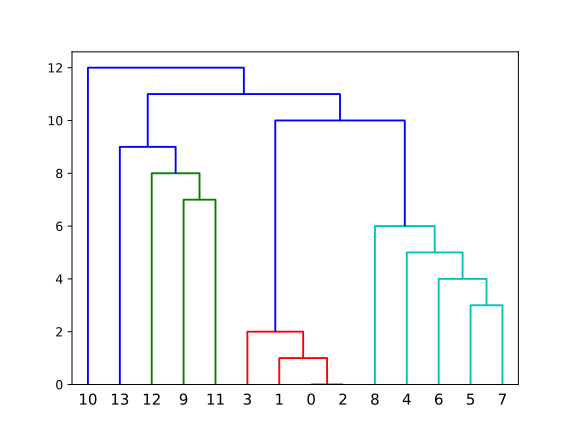
\includegraphics[width=0.49\textwidth]{img/extract_ex_dendro.png}
        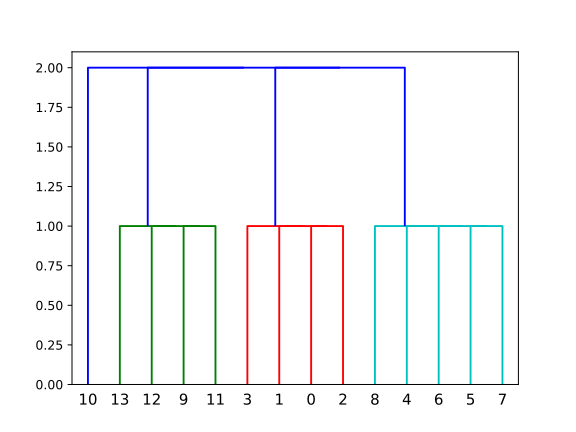
\includegraphics[width=0.49\textwidth]{img/extract_ex_taxo.png}
    \caption{The Input and output of the taxonomy extraction heuristic}
    \label{fig:my_label}
\end{figure}


\section{One-Step Approach}\label{\positionnumber}
Hierarchical clustering algorithms may be divided into \textbf{agglomerative and divisive methods}~\cite{han2011data}. Agglomeraitve methods start with each data instance beeing a cluster and merges in all subsequent steps 2 clusters at a time in a bottom-up fashion. Divisive methods start with all instances beeing in the same cluster and splits them consecutively top-down. We are going to focus on the agglomerative methods as there are computational challenges inherent to divisive clustering that agglomerative clustering does not have\note{There are $2^{n-1}-1$ possible ways to partition a set of n elements into 2 sets and in divisive clustering one needs to heuristically choose a partitioning. Backtracking could improve the performance but this is not scalable and may end up in exponential runtime.\cite{han2011data}}~\cite{han2011data}. \\

\subsection{Hierarchical Agglomerative Clustering}\label{\positionnumber}
Agglomerative methods need a measure for the distance between two clusters. The most common choices are with $C_i, C_j$ clusters:
\begin{itemize}
    \item \textbf{Minimum distance}, also called \textbf{Single Linkage}: 
    \[d_{\text{min}}(C_i, C_j) = \min_{e_1 \in C_i, e_2 \in C_j} |e_1 - e_2|\]
    \item \textbf{Maximum distance}, also called \textbf{Complete Linkage}: 
    \[d_{\text{max}}(C_i, C_j) = \max_{e_1 \in C_i, e_2 \in C_j} |e_1 - e_2|\]
    \item \textbf{Average distance}, also called \textbf{Average Linkage}: 
    \[d_{\text{avg}}(C_i, C_j) = \frac{1}{|C_i| \cdot |C_j|} \sum_{e_1 \in C_i, e_2 \in C_j} |e_1 - e_2|\]
\end{itemize}
There are also the centroid distance, computing the distance from the mean elements of each cluster and Ward's method but those use the notion of the mean element (or the center of gravity of the cluster) which is not directly applicable for binary attributes\note{One could use fuzzy logic in order to provide a mean with non-crisp attributes in order to apply the other two distances~\cite{kruse2016computational}.} \cite{mirkin2013mathematical, han2011data}. A visualization of the distances is shown in fig. \ref{fig:agglo_dist}.
\fig{img/agglo_distance.png}{agglo_dist}{The different distance functions visualized}{1} \\
The algorithm proceeds as follows: 
\begin{enumerate}
    \item initialize all data objects as own clusters
    \item compute the cluster distance matrix by computing the chosen distance function pairwise for all clusters
    \item remove and merge the two clusters with the minimal distance with respect to the chosen distance function. add the new cluster to the list of clusters
    \item if there are more than 2 elements in the set of clusters continue with step 2\note{Alternatively one can specify the amount of clusters desired, but as we are interested in hierarchies here this is not desired.}. This is procedure is neither complete not always correct. For example two clusters differing in a different attribute but still having the distance 1 may be merged. There are also other operations to integrate 
\end{enumerate}
\begin{algorithm}[h]
    \KwIn{A matrix $M$ of shape $|O| \times |A|$ with $m_{o,a} \in \{0, 1\}$ that is consistent with $I$}
    \Parameters{Distance function d}
    \KwOut{A linkage matrix $lM$}
    \Begin{
        List cluster $\rightarrow$ initializeObjectsAsOwnCluster(M)\;
        \While{cluster.size() > 2)}{
            dM $\rightarrow$ computePairwiseDistance(cluster)\;
            m1, m2 $\rightarrow \text{argmin}_{r_1, r_2 \in \text{dM}}(r_1, r_2)$\;
            cluster $\rightarrow (cluster \setminus m1 \setminus m2) \cup (m_1 \cup m_2)$
        }
        return cluster
    }
\caption{Hierarchical Agglomerative Clustering}\label{agglo}
\end{algorithm}

\subsection{Robust Single Linkage}\label{\positionnumber}
% TODO %%%%%%%%%%%%%%%%%%%%%%%%%%%%%%%%%%%%%



\section{Two-Step Approach}\label{\positionnumber}
% TODO %%%%%%%%%%%%%%%%%%%%%%%%%%%%%%%%%%%%%
The two step approaches first use a non-hierarchical algorithm in order to derive basic clusters in order to apply hierarchical clustering atop of the output of the non-hierarchical algorithm. This results not only in a performance gain but also yields a smaller and thus more interpretable dendrogram. In the following a subset of the evaluated algorithms is described. 
\subsection{Non-Hierarchical Clustering}
\subsubsection{K-Medians}\label{\positionnumber}
\subsubsection{TTSAS}\label{\positionnumber}
\subsubsection{Self-organizing Map}\label{\positionnumber}

\subsection{Subsequent Hierarchical Clustering}
This also yields problems: When the first clustering procedure was applied, one needs to (re-)construct a feature description of the cluster so that the hierarchical clustering algorithm can calculate the distance of clusters. One option is to take the intersection of the category sets of the elements in the clusters. Another option is to construct a probabilistic description  of the feature sets. 

\subsection{OPTICS}\label{\positionnumber}
\subsection{HDBSCAN}\label{\positionnumber}



\section{Conceptual Clustering}
\subsection{Trestle}

\section{Implementation}


\section{Evaluation}
 \subsection{Datasets}
   
  \section{Results}
    \subsection{Yelp}
    \subsection{synthetic}



 \chapter{Evaluation}
 \section{Proposed Method: Graph-aware clustering of Nodes}
 
\subsubsection{Cobweb}\label{\positionnumber}
\paragraph{Category Utility}
\paragraph{Concept Representation}
\paragraph{Search and Operators}

\paragraph{Cobweb/3}

\paragraph{Labyrinth}

\subsection{Extracting Structural Features}
\subsubsection{Characteristic Sets}
\subsubsection{Recursive Feature Extraction}
\subsubsection{Role Extraction}

\subsection{The graph-aware pipeline}

\subsubsection{Complexity Analysis}

\section{Implementation Highlights}
For this method i had that challenge "sell yourself"
 
 
 
 \subsection{Setup}
 \subsubsection{Datasets}
 \subsubsection{Ground Truth}
   
  \subsection{Results}
    \subsubsection{Yelp}
        \paragraph{Object-based}
        \paragraph{Graph-based}
        
    \subsubsection{LDBC SNB}
\chapter{Conclusion}
\section{Applications}
% include dep type system in Leo's cypher compiler
% derive types from unstructured dbs to gen rdbms schemas
% cluster types of events with value based method

\section{Future Work}
% take input from classifier, do uncertainty based clust, use prob. dep. ts
% same for edges

\section{Summary}



\newgeometry{left=2.5cm, right=2.5cm, bottom=2cm, top=2.5cm,headheight=12pt, headsep=0.8cm, footskip=22pt}
\chapter{Appendix}

\section{Taxonomy Extraction example}
\begin{minipage}{0.4\textwidth}
$C_{14} = C_0 \cup C_2$, with distance 1 \\
$C_{15} = C_1 \cup C_14$, with distance 1 \\
$C_{16} = C_3 \cup C_15$, with distance 1 \\
$C_{17} = C_5 \cup C_7$, with distance 1 \\
$C_{18} = C_6 \cup C_17$, with distance 1 \\
$C_{19} = C_4 \cup C_18$, with distance 1 \\
$C_{20} = C_8 \cup C_19$, with distance 1 \\
$C_{21} = C_9 \cup C_11$, with distance 1 \\
$C_{22} = C_12 \cup C_21$, with distance 1 \\
$C_{23} = C_13 \cup C_22$, with distance 1 \\
$C_{24} = C_16 \cup C_20$, with distance 2 \\
$C_{25} = C_23 \cup C_24$, with distance 2 \\
$C_{26} = C_10 \cup C_25$, with distance 2 \\
\end{minipage} \hfill
\begin{minipage}{0.4\textwidth}
$[[ 0.  2.  1.]$ \\
 $[ 1. 14.  1.]$\\
 $[ 3. 15.  1.]$\\
 $[ 5.  7.  1.]$\\
 $[ 6. 17.  1.]$\\
 $[ 4. 18.  1.]$\\
 $[ 8. 19.  1.]$\\
 $[ 9. 11.  1.]$\\
 $[12. 21.  1.]$\\
 $[13. 22.  1.]$\\
 $[16. 20.  2.]$\\
 $[23. 24.  2.]$\\
 $[10. 25.  2.]]$ \\
\end{minipage} \\

\begin{minipage}{0.4\textwidth}
$[$\\
    $[[ 0.  2.  1.  3.], 1]$\\
    $[[ 5.  7.  6.  4.  8.], 1]$\\
    $[[ 9. 11.  12.  13. ], 1]$\\
    $[[16.  20.  23.  10.], 2]$  \\        
$]$\\
\end{minipage}  \hfill
\begin{minipage}{0.4\textwidth}
$C_{16} = C_0 \cup C_2 \cup C_1 \cup C_3$, with distance 1 \\  
$C_{20} = C_5 \cup C_7 \cup C_6 \cup C_4 \cup C_8$, with distance 1 \\ 
$C_{23} = C_9 \cup C_{11} \cup C_{12} \cup C_{13}$, with distance 1 \\ 
$C_{26} = C_{16} \cup C_{20} \cup C_{23} \cup C_{19}$, with distance 2 \\         
\end{minipage} 
\printbibliography
\end{document}
